\documentclass[conference]{IEEEtran}

\usepackage[T1]{fontenc}
\usepackage[utf8]{inputenc}
\usepackage{graphicx}
\usepackage{booktabs}
\usepackage{multirow}
\usepackage{amsmath}
\usepackage{url}
\usepackage{xcolor}
\usepackage{hyperref}
\hypersetup{hidelinks}

\title{PhasePhyto: A Rigorous OOD Study of Physics-Informed Fusion for Botanical Image Classification}

\author{%
\IEEEauthorblockN{Matheshwara Annamalai Senthilkumar, Arunbh Yashaswi}
\IEEEauthorblockA{Group 25\\
University of Maryland, Baltimore County\\
UID: 121281500, 121304537}
}

\begin{document}
\maketitle

\begin{abstract}
This project studies out-of-distribution (OOD) plant disease classification using PlantVillage as the source domain and PlantDoc as the target domain~\cite{Hughes2015,Singh2020}. We developed \textit{PhasePhyto}, a three-stream architecture that combines phase congruency features, a ViT-B/16 semantic backbone, and a CLAHE-based illumination stream through cross-attention. The original hypothesis was that phase congruency's formal amplitude invariance would improve transfer from clean laboratory imagery to cluttered field imagery. Our controlled ablation study shows that this hypothesis is not supported: the full model and a backbone-only variant achieve identical target accuracy (0.5229), while the phase-congruency-only variant collapses to near-random target performance (macro-F1 0.0791). However, the broader OOD recipe---label smoothing, differential learning rates, EMA, SAM, strong augmentation, HSV foreground gating, horizontal-flip TTA, and TENT---improves the target accuracy of the system from 47.71\% to 52.29\%. A second strict apple-overlap benchmark on PlantVillage, PlantDoc, and Plant Pathology 2021 further shows that softened class rebalancing is more effective than post-hoc calibration, raising PP2021 macro-F1 from 0.6813 to 0.7015. The final outcome is therefore both a negative result on the architectural claim and a practical recipe for stronger botanical transfer under domain shift.
\end{abstract}

\section{Introduction}
Plant disease classifiers often perform extremely well on curated benchmark data but degrade sharply when deployed in real field conditions. This project focuses on the PlantVillage $\rightarrow$ PlantDoc setting~\cite{Hughes2015,Singh2020}, where the source domain contains isolated leaves with uniform backgrounds and stable lighting, while the target domain contains clutter, occlusion, viewpoint changes, and severe illumination variation. The resulting generalization gap is large enough that it serves as a useful benchmark for studying OOD robustness rather than only in-distribution accuracy.

Our initial hypothesis was inspired by image phase congruency (PC), a frequency-domain feature operator that measures local phase alignment and is formally invariant to monotonic amplitude scaling~\cite{Kovesi1999}. Intuitively, this suggested that PC might capture structural lesion boundaries in a way that is less sensitive to lighting changes than raw RGB intensities. We therefore built a fusion architecture that explicitly combines physics-informed structural cues with a strong pretrained semantic backbone.

The project ultimately became a controlled empirical study of what does and does not transfer OOD. Two guiding questions remained central throughout: \emph{(1) does PC fusion help plant-disease transfer under domain shift?} and \emph{(2) which practical training interventions produce reliable gains even if the original architecture hypothesis fails?} The answer to the first question is negative on our benchmark; the answer to the second is positive, and it yields the main practical contribution of the work.

\section{Methodology}
\subsection{PhasePhyto Architecture}
PhasePhyto uses three streams. The first converts the input image to grayscale, applies a log-Gabor filter bank, and derives three structural maps: PC magnitude, phase symmetry, and oriented energy. A lightweight CNN encoder converts these into structural tokens. The second stream uses a pretrained ViT-B/16 backbone to produce semantic tokens from the RGB image. The third stream applies CLAHE-based illumination normalization and a shallow CNN to produce an auxiliary illumination vector. In the full model, structural tokens query semantic tokens through cross-attention, and the fused representation is concatenated with the illumination vector before classification.

This design was intended to embed a physics-based inductive bias directly into the model rather than relying only on learned invariance from augmentation. The PC branch is especially appealing in theory because it has no trainable filters at the feature-extraction stage: the log-Gabor bank is fixed, and only the downstream token encoder and fusion module are learned.

\subsection{Controlled Ablation Design}
To isolate the architectural contribution, we held the training recipe fixed and compared four forward-path ablations:
\begin{itemize}
    \item \textbf{full}: PC + ViT + CLAHE with cross-attention fusion
    \item \textbf{backbone\_only}: ViT + CLAHE only
    \item \textbf{no\_fusion}: PC + ViT + CLAHE without cross-attention
    \item \textbf{pc\_only}: PC + CLAHE only
\end{itemize}
This makes it possible to determine whether the PC stream itself helps, whether cross-attention adds value, and whether observed gains are architectural or instead come from the training recipe.

\subsection{Training Recipe}
The most effective configuration used label smoothing ($\epsilon=0.1$)~\cite{Szegedy2016}, differential learning rates with a lower backbone multiplier, exponential moving average (EMA)~\cite{Izmailov2018}, Sharpness-Aware Minimization (SAM)~\cite{Foret2021}, RandAugment~\cite{Cubuk2020}, shared-mask random erasing~\cite{Zhong2020}, HSV-masked background replacement, HSV leaf foreground gating, horizontal-flip test-time augmentation, and TENT adaptation at evaluation time~\cite{Wang2021}. These choices were motivated by a practical goal: reduce source overfitting while improving tolerance to target-domain clutter and lighting noise.

\subsection{Datasets and Evaluation}
The primary benchmark uses PlantVillage as source and PlantDoc as target with a 25-class mapped label space and a target test set of 153 images. We report source accuracy/F1 and target accuracy/macro-F1. Because the target set is small, we also designed a stricter follow-up benchmark on the shared 3-class apple label space across PlantVillage, PlantDoc, and Plant Pathology 2021 (PP2021). This overlap benchmark provides a much larger real-world target set (n = 11{,}310) and lets us test whether observed failure modes are due mainly to class-prior mismatch or to genuine feature shift.

\section{Results}
\subsection{Main 25-Class OOD Ablation}
Table~\ref{tab:ablation} summarizes the central ablation result.

\begin{table}[ht]
\caption{PlantVillage $\rightarrow$ PlantDoc ablation results (target metrics include TTA+TENT).}
\label{tab:ablation}
\centering
\begin{tabular}{lcccc}
\toprule
Ablation & Src Acc & Src F1 & Tgt Acc & Tgt F1 \\
\midrule
full+leafmask & 0.9975 & 0.9955 & 0.5229 & 0.3944 \\
backbone\_only & 0.9975 & 0.9955 & 0.5229 & 0.3859 \\
no\_fusion & 0.9975 & 0.9955 & 0.4902 & 0.3464 \\
pc\_only & 0.7340 & 0.5878 & 0.0915 & 0.0791 \\
\bottomrule
\end{tabular}
\end{table}

The key observation is that \textbf{full} and \textbf{backbone\_only} achieve identical target accuracy and differ by only +0.009 macro-F1. Under a shared recipe, the PC stream therefore does \emph{not} deliver a meaningful OOD gain over the semantic backbone. In contrast, \textbf{pc\_only} fails dramatically on target data despite carrying nontrivial source signal, which immediately suggests that feature-level invariance is insufficient for robust classifier-level transfer.

\begin{figure*}[t]
    \centering
    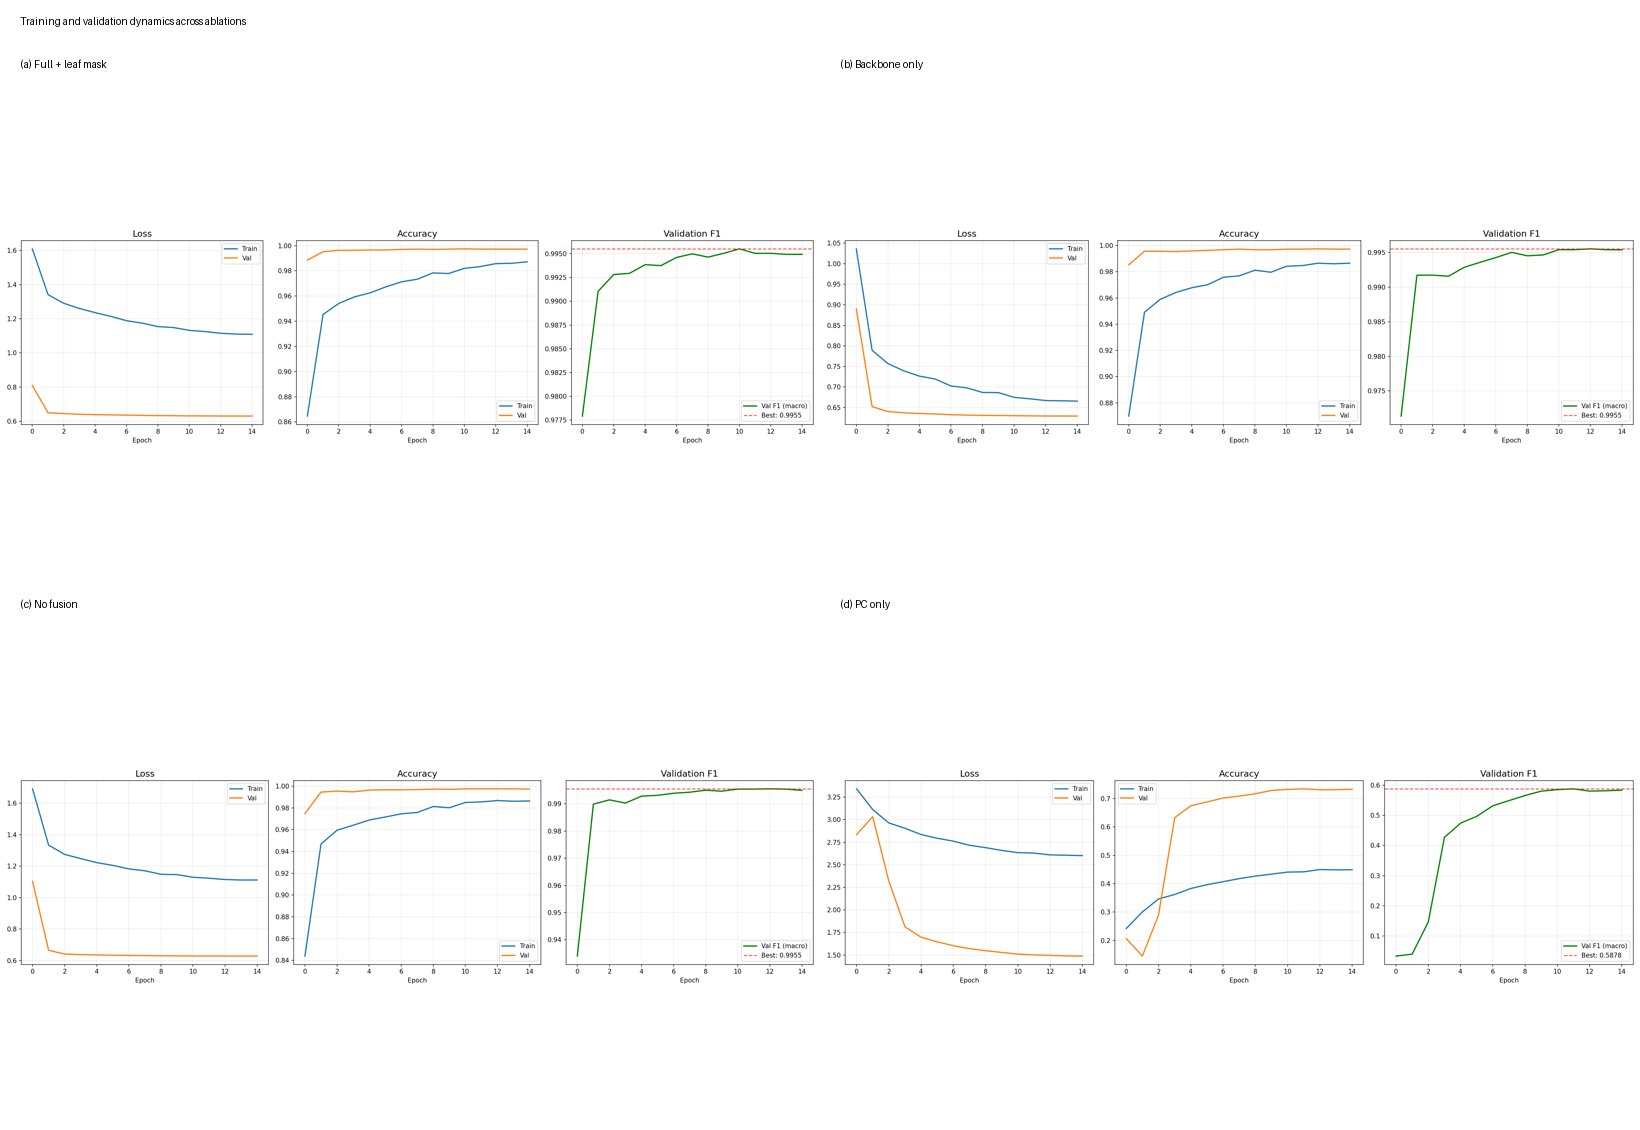
\includegraphics[width=\textwidth]{figures/ablation_training_grid.png}
    \caption{Training and validation dynamics across the four ablations. The full and backbone-only variants converge to similarly strong source performance, while the PC-only branch saturates early and never approaches competitive validation quality.}
    \label{fig:traininggrid}
\end{figure*}

Figure~\ref{fig:traininggrid} reinforces this interpretation. The full, backbone-only, and no-fusion variants all fit the source domain easily, but only the semantic-path variants maintain strong target transfer. The PC-only branch shows a lower ceiling even on source training, and the resulting target breakdown confirms that the structural stream alone is not sufficiently discriminative under field shift.

\subsection{Recipe-Driven Improvement}
Although the architectural claim was not validated, the training recipe itself improved target performance. Relative to the earlier plain-recipe baseline (47.71\% target accuracy, 0.3603 macro-F1), the final hardened configuration reached 52.29\% target accuracy and 0.3944 macro-F1. This is a gain of +4.6 percentage points in target accuracy and +3.4 points in target F1. The most defensible practical claim of the project is therefore not ``PC fusion wins,'' but rather that a carefully layered OOD recipe materially improves transfer on this benchmark.

\begin{figure*}[t]
    \centering
    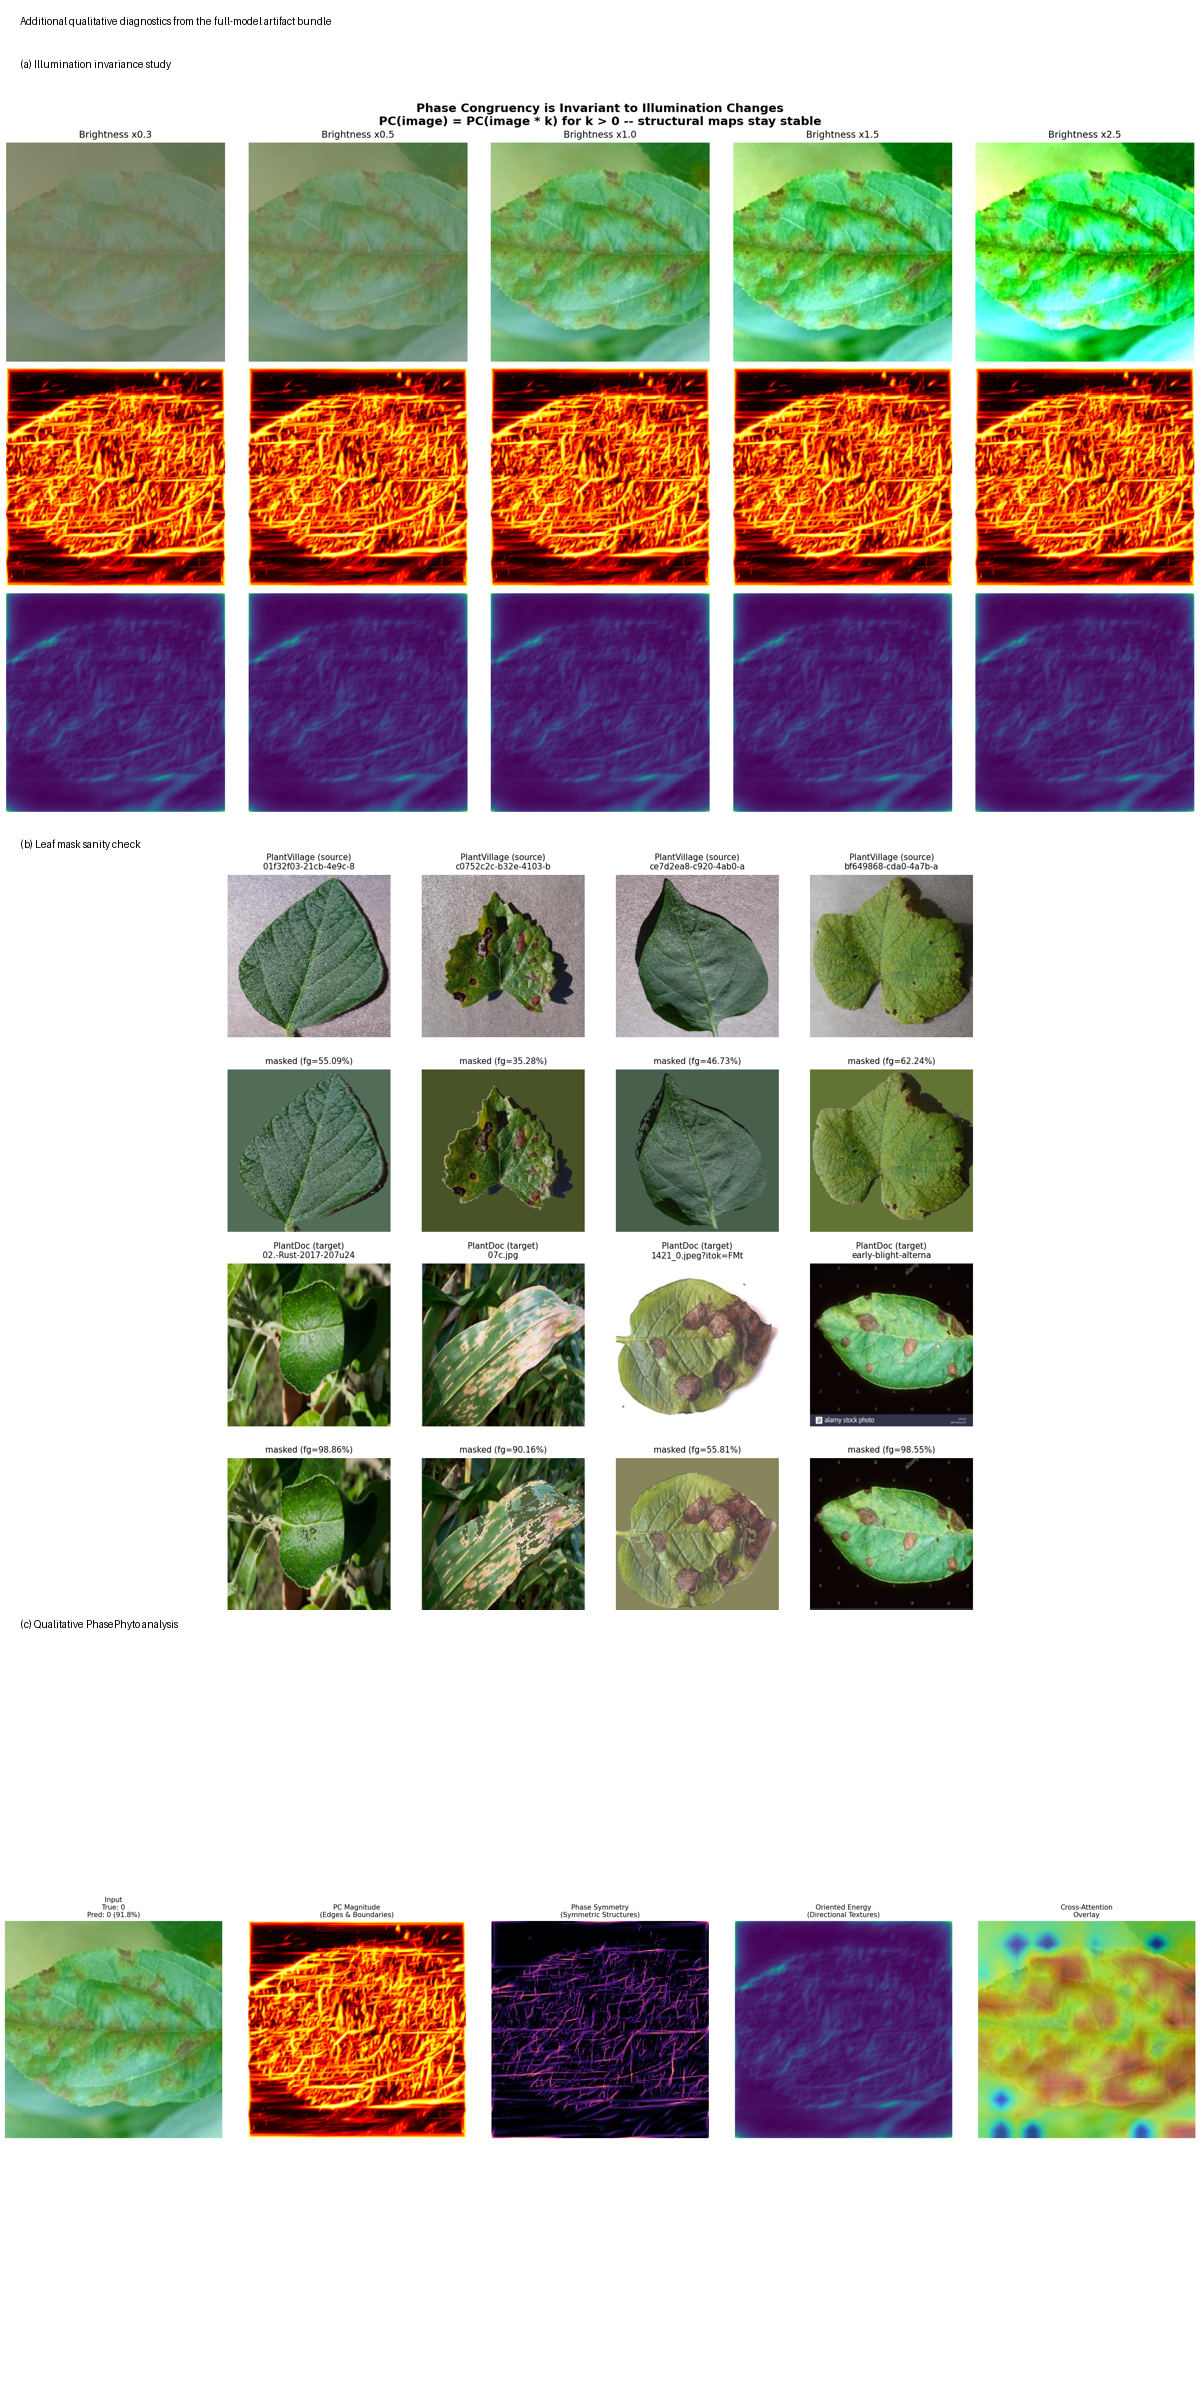
\includegraphics[width=\textwidth]{figures/phasephyto_diagnostics_grid.png}
    \caption{Additional diagnostics from the full-model artifact bundle. The illumination-invariance panel shows how frequency-domain maps remain structured under brightness changes; the leaf-mask sanity panel shows the gating used to suppress background clutter; the qualitative analysis panel visualizes PC maps and attention behavior on a representative sample.}
    \label{fig:diagnostics}
\end{figure*}

The diagnostic panels in Figure~\ref{fig:diagnostics} help explain why the recipe remains useful even though the full fusion model does not outperform the backbone-only baseline. The illumination and leaf-masking utilities still suppress nuisance variation, and the attention visualizations show that the model does respond to biologically meaningful structure. The negative result is therefore not ``the model learned nothing,'' but rather ``the extra structural branch did not convert those signals into measurable OOD gains over a strong ViT baseline.''

\begin{figure}[t]
    \centering
    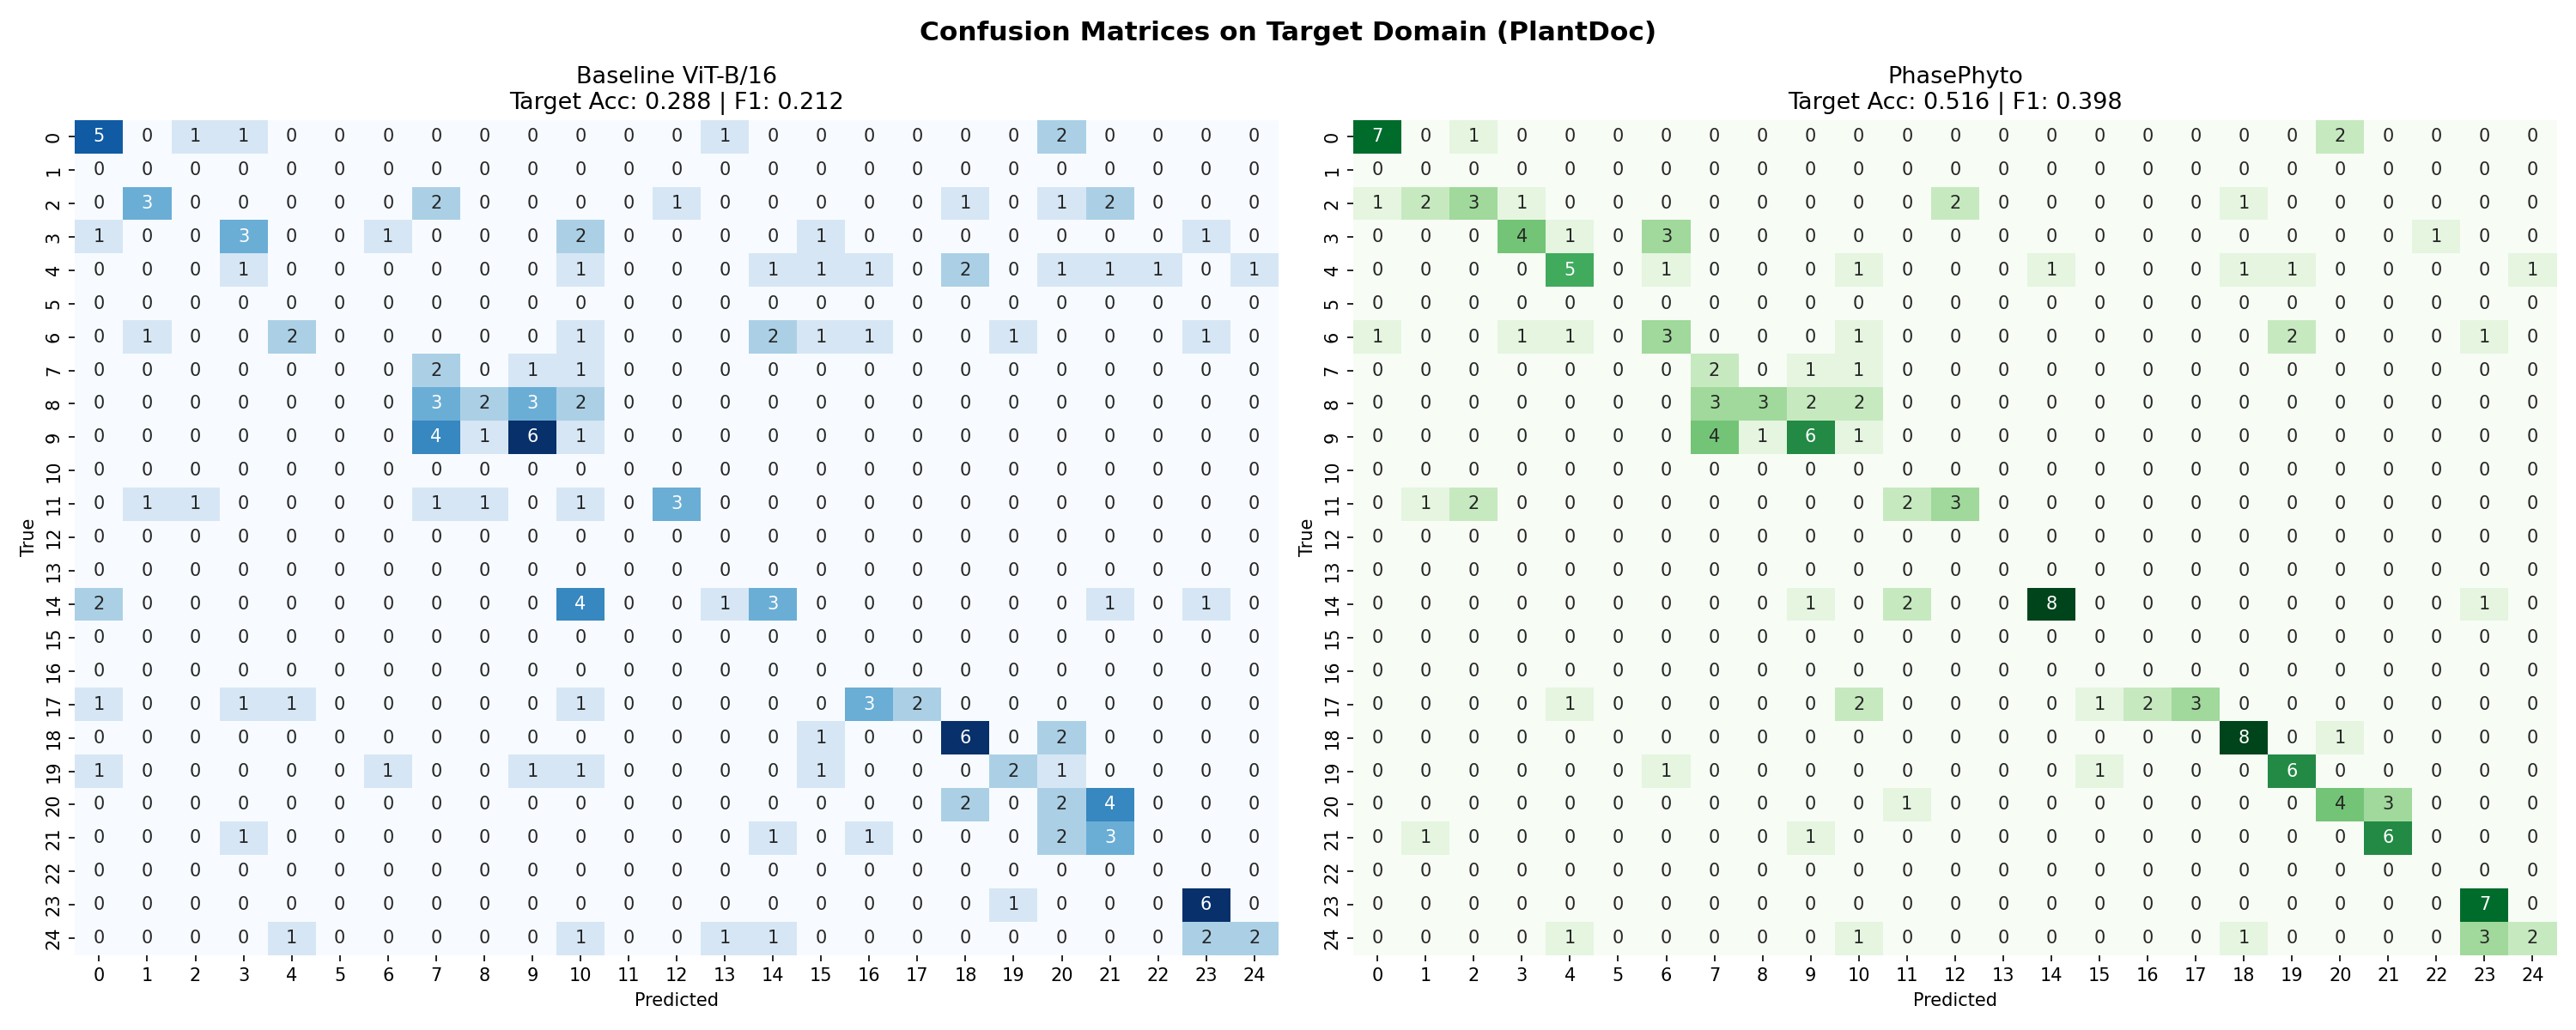
\includegraphics[width=\linewidth]{figures/confusion_matrices.png}
    \caption{Source and target confusion-matrix comparison for the final full-model artifact bundle. The strong source performance contrasts sharply with the noisier target confusion pattern.}
    \label{fig:confusion}
\end{figure}

The confusion matrices in Figure~\ref{fig:confusion} make the source--target gap visually explicit. Source predictions are nearly saturated, whereas the target confusion pattern remains diffuse, supporting the claim that the unresolved problem is domain shift rather than underfitting.

\subsection{Strict Apple-Overlap Benchmark}
To test whether the main story survives under tighter label control, we built a second benchmark on the shared 3-class apple label space (healthy, apple scab, cedar apple rust) across PlantVillage, PlantDoc, and PP2021. This removes the ``label mismatch is doing the work'' explanation and provides a statistically meaningful real-world target set.

\begin{figure}[t]
    \centering
    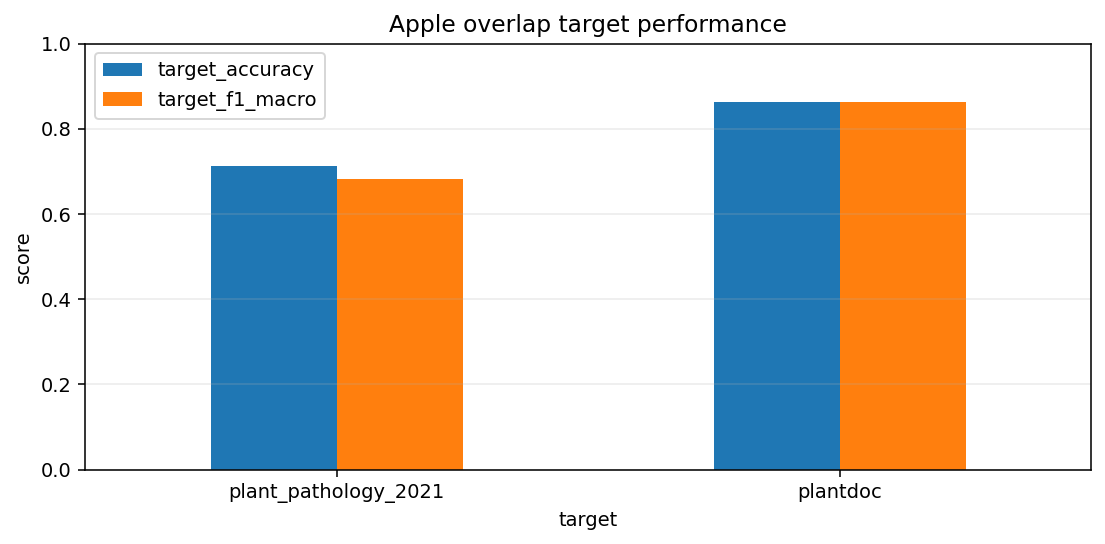
\includegraphics[width=\linewidth]{figures/apple_overlap_summary.png}
    \caption{Baseline apple-overlap summary across PlantDoc and PP2021. The PP2021 gap is much larger and therefore more informative than the small PlantDoc test split.}
    \label{fig:appleoverlap}
\end{figure}

On PP2021, the baseline overlap model reaches 0.7136 accuracy and 0.6813 macro-F1. The target gap is highly asymmetric: healthy remains relatively strong, while apple scab and especially cedar apple rust degrade sharply. This exposes two failure modes: a \emph{healthy bias} induced by the PlantVillage class prior and a \emph{rust$\rightarrow$scab visual collapse} that calibration alone cannot fix.

For completeness, the same source-only model reaches 0.8621 accuracy and 0.8632 macro-F1 on the much smaller PlantDoc apple-overlap split. We treat that result as directionally useful but statistically anecdotal because the target sample size is only $n=29$.

\begin{table}[t]
\caption{PP2021 follow-up interventions on the apple-overlap benchmark.}
\label{tab:fixes}
\centering
\begin{tabular}{lcc}
\toprule
Variant & Accuracy & Macro-F1 \\
\midrule
Baseline & 0.7136 & 0.6813 \\
Fix A uniform prior & 0.6789 & 0.6619 \\
Fix A oracle prior & 0.7049 & 0.6779 \\
Fix B full rebalance & 0.7416 & 0.6969 \\
Fix B softer rebalance & \textbf{0.7393} & \textbf{0.7015} \\
\bottomrule
\end{tabular}
\end{table}

Table~\ref{tab:fixes} shows that the best-performing intervention is not calibration but softer class rebalancing (\texttt{balanced\_sampler\_power = 0.5}). Even oracle-prior calibration underperforms the baseline on macro-F1, which is strong evidence that the residual gap is not mainly a prior-shift problem.

\begin{figure}[t]
    \centering
    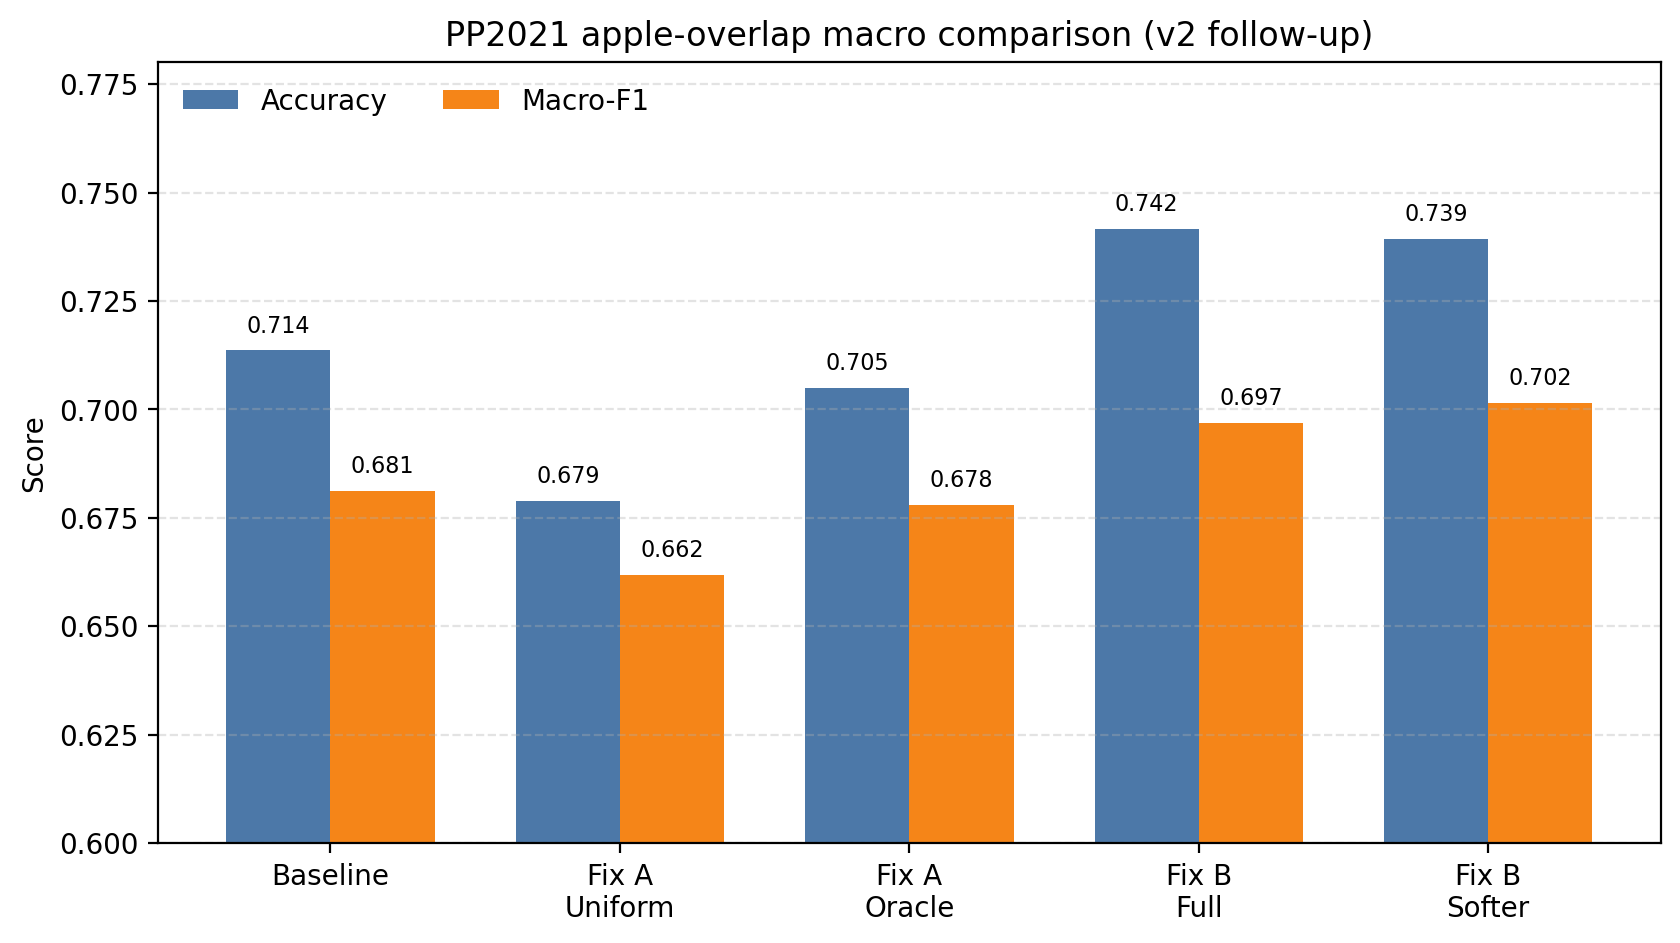
\includegraphics[width=\linewidth]{figures/pp2021_macro_comparison_v2.png}
    \caption{PP2021 macro comparison for the v2 apple-overlap follow-up. Softer rebalancing provides the strongest macro-F1 while maintaining high accuracy.}
    \label{fig:ppmacro}
\end{figure}

Figure~\ref{fig:ppmacro} highlights the macro trend clearly. Fix A with a uniform target prior is net harmful, oracle-prior Fix A is still slightly below baseline, and both rebalancing variants improve overall transfer. The softer rebalancing setting trades a tiny amount of accuracy for the best macro-F1, which is the more appropriate metric under class asymmetry.

\begin{figure}[t]
    \centering
    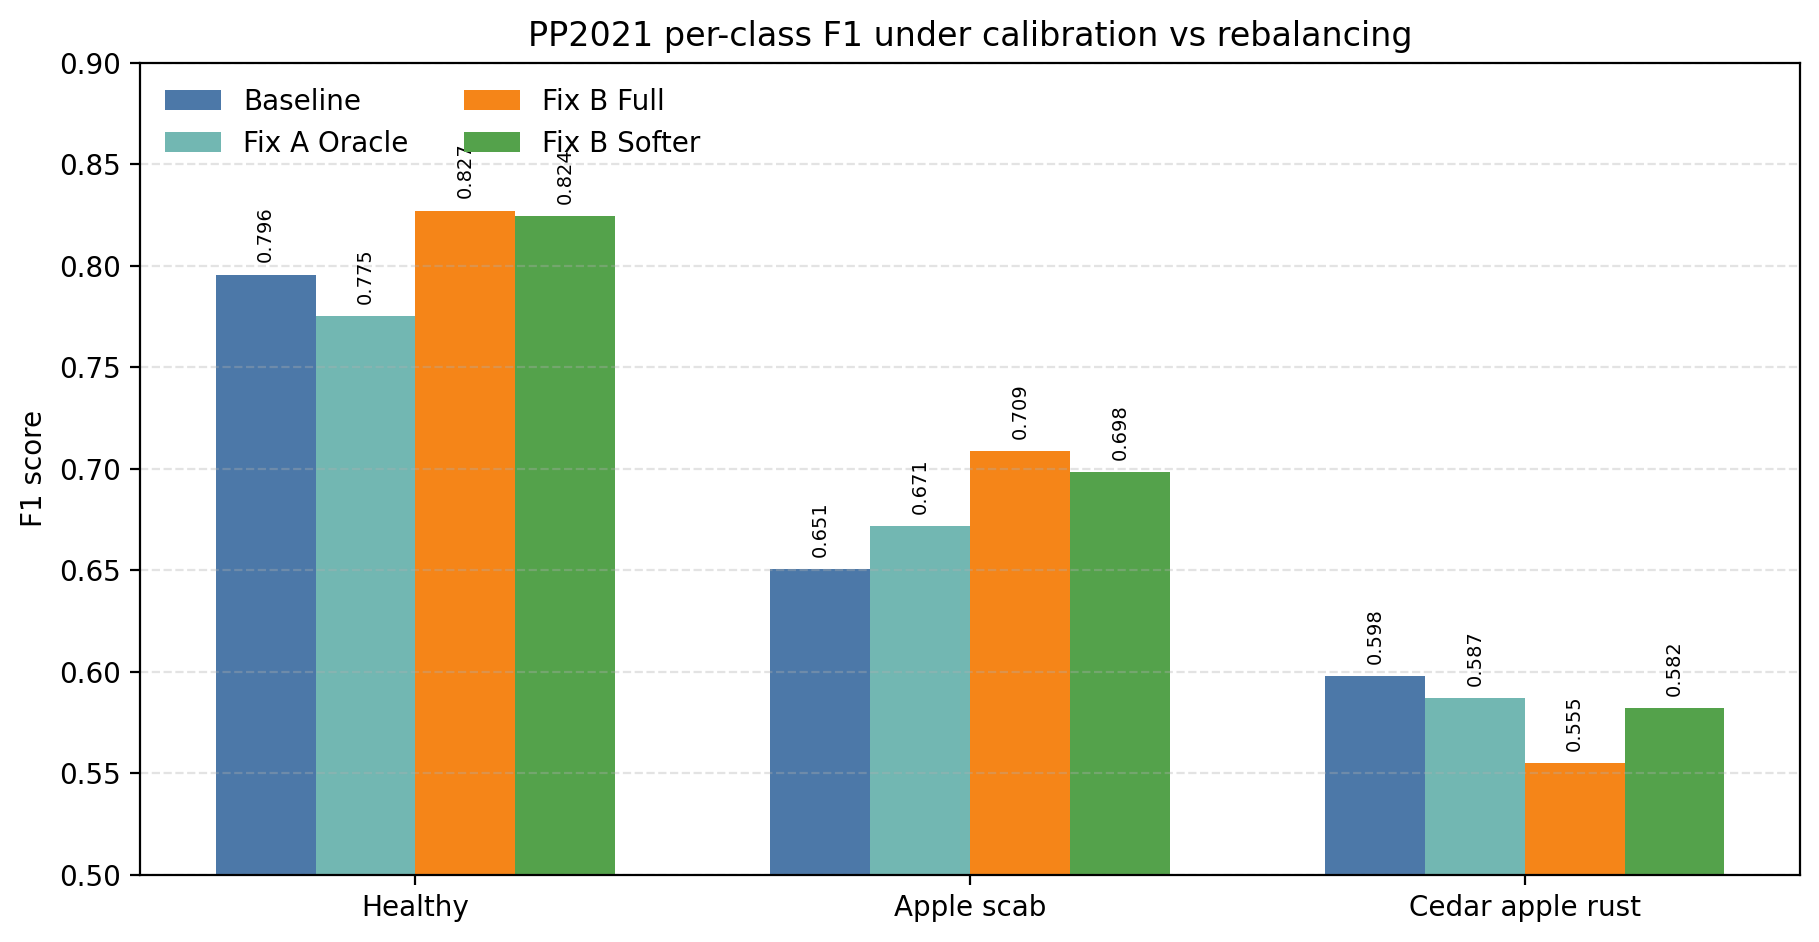
\includegraphics[width=\linewidth]{figures/pp2021_per_class_f1_v2.png}
    \caption{Per-class PP2021 F1 under calibration and rebalancing. The main win from rebalancing is stronger scab/healthy balance, while calibration does not recover the rust-specific feature-shift problem.}
    \label{fig:ppclassf1}
\end{figure}

Per-class F1 in Figure~\ref{fig:ppclassf1} clarifies why the softer rebalancing variant is preferable. Full rebalancing gives the best scab F1 but harms rust too aggressively: cedar apple rust drops from 0.5977 at baseline to 0.5551 under full rebalancing. The softer setting raises rust back to 0.5820 while preserving strong healthy and scab performance, so it recovers most of the rust regression without giving up the macro-level gain.

\section{Discussion}
The main scientific finding is a negative one: \emph{amplitude-invariant features are not automatically classifier-invariant}. The PC operator itself satisfies the invariance property it was designed for~\cite{Kovesi1999}, but the learned classifier can still overfit source-specific structure embedded in those invariant features. Our experiments therefore point to what we call the \emph{invariance--classifier-head gap}: mathematically stable local features do not guarantee stable downstream decision boundaries.

The ablations also clarify the role of fusion. Removing cross-attention while keeping the PC stream (\textbf{no\_fusion}) hurts target performance more than removing the PC stream altogether (\textbf{backbone\_only}). This suggests that the fusion mechanism can sometimes mitigate damage introduced by the structural branch, but it does not create new transfer signal strong enough to beat the semantic backbone. In other words, cross-attention behaves more like a stabilizer than like a decisive OOD advantage.

The apple-overlap follow-up sharpens the practical lesson. Because calibration fails even under oracle priors, the dominant error source is not just a mismatched class distribution. Instead, the residual gap contains a genuine feature-shift component, especially visible in the rust/scab confusion. That is why recipe-side interventions such as softer rebalancing help more than post-hoc calibration: they reshape the learned boundary during training rather than only shifting logits after the fact.

There are still limitations. The main 25-class PlantDoc target set contains only 153 mapped samples, so tiny deltas should not be over-interpreted. The overlap study is stronger because PP2021 provides n = 11{,}310 target samples, but it is still based on a single-seed sweep. A natural next step would be multi-seed confirmation plus a transductive intervention such as TENT on PP2021 or a small target fine-tune. Those experiments would test whether the remaining rust-specific gap is mostly adaptation-limited rather than architecture-limited.

\section{Conclusion}
This project developed and evaluated PhasePhyto, a physics-informed fusion architecture for botanical OOD classification. The final ablation results show that the original architectural claim does not hold on the PlantVillage $\rightarrow$ PlantDoc benchmark: the full model does not beat an equally trained backbone-only model in a meaningful way, and the PC-only variant fails dramatically on the target domain. However, the project still delivers a useful practical contribution: a reproducible OOD recipe, a rigorous ablation methodology, and a second overlap benchmark that decomposes prior shift from feature shift. The broader lesson is that formal invariance in feature extraction does not guarantee OOD robustness at the classifier level, and that careful empirical discipline is essential when evaluating physics-inspired neural architectures.

\section*{Acknowledgments}
We thank the course staff and dataset creators whose resources made this project possible. We also acknowledge the publicly available PlantVillage, PlantDoc, and Plant Pathology 2021 datasets, as well as the open-source PyTorch, timm, Streamlit, Docker, and Hugging Face ecosystems used in the implementation and deployment workflow.

\bibliographystyle{IEEEtran}
\bibliography{references}

\end{document}
